\section{Background}
The target audiences of the proposed tool are domain experts who analyze and develop NLP models. Therefore, certain background knowledge in NLP is required to fully understand and appreciate the technique discussed in this paper. In this section, we first explain the definition of natural language inference (NLI) task and how it fits into the grand challenges in NLP. Then, we examine the common architectural characteristics shared by many state-of-the-art neural network models. Finally, we discuss the role attention plays in the model and why attention is closely tied to model interpretability.

\subsection{Natural Language Inference}
\label{sec:languageInference}
Natural Language Inference (NLI)~\cite{DaganRothSammons2013} is an important machine understanding task in NLP.
The goal of NLI is to predict the relationship between a premise (\textbf{P}) sentence and a hypothesis (\textbf{H}) sentence.
The prediction falls in one of three categories: \emph{entailment} (\textbf{E}), \emph{contradiction} (\textbf{C}), and \emph{neutral} (\textbf{N}).
A simple example is shown in Table~\ref{tab:NLI}.
In this case, the premise is ``Boy ate an apple''.
The hypothesis statement ``Kid ate fruits'' can be concluded from the premise. Therefore, the relationship between the premise and hypothesis is \emph{entailment}. However, we should note that such a relationship is not necessarily reversible. Since the concept ``fruit'' is less restrictive than that of ``apple'', we cannot conclude ``Boy ate an apple'' from the statement ``Kid ate fruit''. The same logic applies to the hypothesis of ``Boy ate a Fuji apple.'', in which the premise neither implies nor opposes the hypothesis, and therefore, their relationship is \emph{neutral}.
%\emph{Contradiction} means the textual of hypothesis opposes that of premise;
%and \emph{Neutral} implies no conclusion can be made on either \emph{Entailment} or \emph{Contradiction}.

\begin{table}[htbp]
\vspace{-2mm}
\label{tab:NLI}
\centering
\caption{An illustration of natural language inference.}
 \begin{tabular}{c | c c c c}
 \hline
  P / H & sentences & entail & contradict & neutral \\ [0.5ex]
 \hline
 premise & Boy ate an apple. &  -  &  -  & - \\
 hypothesis & Kid ate fruits. & \checkmark &   &  \\
 hypothesis & Boy ate a banana. &  & \checkmark & \\
 hypothesis & Tom ate an apple. &  &  & \checkmark \\
 hypothesis & Boy ate a Fuji apple. &   &  & \checkmark \\
 %\hline
 %premise & Facebook's IPO electrified the general public. &  -  &  -  & - \\
 %hypothesis & Facebook went public. & \checkmark   &  &  \\
 %hypothesis & General Electric went public. &  &   & \checkmark \\
 %hypothesis & People ignored Facebook's IPO. &  & \checkmark & \\
 \hline
\end{tabular}
\vspace{-2mm}
\end{table}


At first glance, the task of natural language inference may seem less practical compared to other well-known NLP challenges such as machine translation; however, the ability to distinguish entailment and contradiction relationship is fundamental to understanding natural language at large.
%
Considering the ambiguousness of natural language and polysemy words, the inference task can become quite challenging (especially from the learning algorithm's point of view). Take the following sentences as an example (here \textbf{P} refers to premise, \textbf{H} refers to hypothesis):  (\textbf{P}) Facebook's IPO electrified the general public; (\textbf{H1}) Facebook went public; (\textbf{H2}) General Electric went public; (\textbf{H3}) People ignored Facebook's IPO. The literal similarity between ``Electric'' and ``electrified'' may trick a model to predict \textbf{H2} as \emph{entailment}. A model likely will also fail to understand the link between ``went public'' and ``IPO'', and therefore, mistake \textbf{H1} as \emph{neutral}.
%
%The grand challenge in Natural Language Processing (NLP) is to have machine to acquire
%deep comprehension of textual information. Major tasks include Natural Language Inference,
%Machine Translation, Questions Answering, Summarization, and etc.
%Recently, neural networks models have performed strongly on these tasks.
%
Recently, Bowman et al. introduced a large corpus~\cite{BowmanAngeliPotts2015} for NLI tasks, which has helped spawn a new wave of effective neural network models for those tasks. Here, we focus on the analysis of the decomposable attention model~\cite{parikh2016emnlp} on this dataset.

% Recently, with the wide adoption of long-short term memory
% (LSTM) network and the introduction of attention mechanism,
% neural network based model have dominated nearly all linguistic tasks
% and thoroughtly refreshed many baseline performances.
% %
% However, the disruptive advance also brings enormous challenges.
% Netural network work based on has long been critizied for their opaque nature,
% and often been regarded as back box approach.
% Due to the opaque nature of the neural network model, interpret and making sense
% of many internal model mechanisms can be extremely challenging.

% \subsection{Neural Network Primer}

\subsection{Neural Network Model in NLP}
%\shusen{What is the basic understanding of neural network What is the end-to-end}
There are many connections and distinctions between neural network models employed for vision and NLP tasks.
On the one hand, as discussed in the introduction, the discrete nature of words and sentences presents additional challenges for
interpreting the NLP model.
%
On the other hand, a majority of recent NLP neural networks share the nature of
end-to-end models, where the entire model operates as a black-box that takes
vectorized input and yields a final prediction for a specific task.
%

Many of the recent NLP end-to-end neural network models, despite having potentially drastically different network architectures, share a similar high-level design that consists of three distinct stages (encode, align, classify, see Fig.~\ref{fig:modelPipeline}).
%
The existence of shared conceptual structures means the proposed tool, although designed for NLI tasks, can be readily generalized for a much broader set of applications.

\begin{figure}[htbp]
\vspace{-2mm}
\centering
 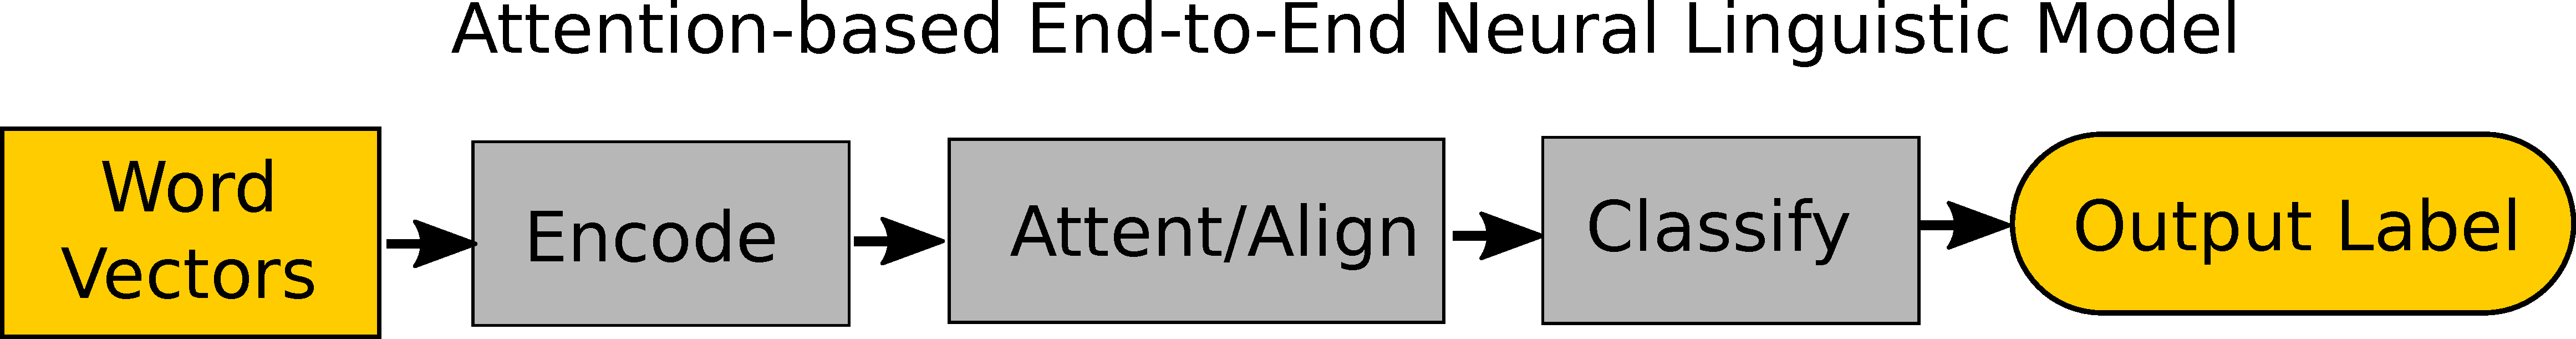
\includegraphics[width=1.0\linewidth]{end2end}
 \vspace{-5mm}
 \caption{The shared structure of end-to-end NLP neural network models.}
  \vspace{-2mm}
\label{fig:modelPipeline}
\end{figure}

These end-to-end models usually take pre-trained word vectors (numerical vector representation of individual words, in which the semantic similarities are expressed by distances in the high-dimensional vector space~\cite{MikolovSutskeverChen2013, PenningtonSocherManning2014}) as input, and then in the encoding stage, the pre-trained vectors are adjusted to the specialized task at hand. Subsequently, the next stage aims at finding alignment between words in the input sequences. For the NLI task, this means finding the correspondance between words from the premise sentence to the hypothesis sentence (see details in Fig.~\ref{fig:attention} and Section~\ref{sec:attention}). Finally, in the last stage, the alignment information and the encoded vector representations are aggregated and then used as features for a classification network (last part of the end-to-end neural network).
%
Since all these three stages of the model are trained jointly in an end-to-end fashion, it is important to explore the interaction between intermediate representations and predictions to make sense of how predictions are made inside such a model.

\subsection{Attention Mechanism}
\label{sec:attention}
Among the three stages, the second stage often constitutes a crucial part of the model as it determines where the classifier will focus for generating a prediction. The operation to compute the alignment between words in the input is referred to as the attention mechanism. 
The introduction of the attention mechanism~\cite{bahdanau2014neural} allows
pairwise interaction between internal representations of words. 
This interaction can be naturally explained as a form of alignment that exposes an interpretable layer in end-to-end neural networks.
%
%As the only interpretable part of the internal state of the network, understanding how attention information 
Recently, attention has contributed to many strongly performed NLP models~\cite{parikh2016emnlp,rush2015neural,yang2016hierarchical,seo2016bidirectional,schwartz2017high}.

\begin{figure}[htbp]
\centering
\vspace{-2mm}
 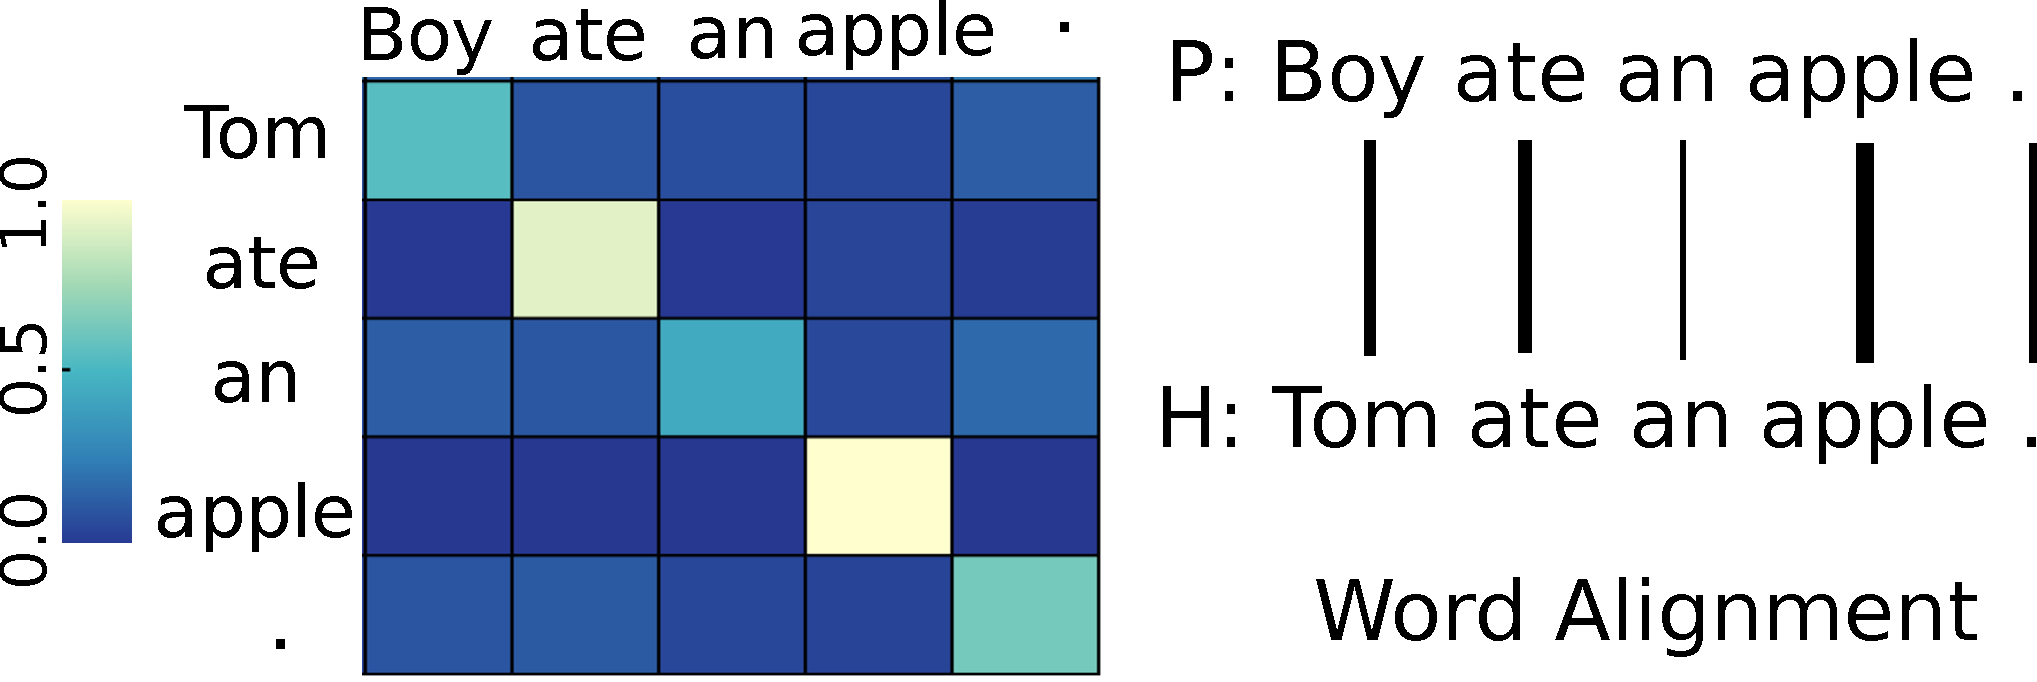
\includegraphics[width=0.9\linewidth]{attentionIllustration}
  \vspace{-2mm}
 \caption{Attention can be naturally explained as a form of alignment which exposes an interpretable layer in end-to-end neural networks. On the left, the matrix shows the attention between between premise and hypothesis pair. On the right, attention can also be interpreted as alignment.}
\label{fig:attention}
  \vspace{-2mm}
\end{figure}

For natural language inference task, as illustrated in Fig.~\ref{fig:attention}, the attention information can be represented as a matrix describing the soft alignment between words in the premise and the words in the hypothesis. As we can see in this example, the higher values indicate significant alignments between words. The \emph{subject}, \emph{verb}, and \emph{object} between these two sentences are aligned correctly (words, such as ``an'', which has less importance in determining sentence relationship, was assigned a lower score). Interestingly, the difference between the subject words does not affect their alignment. The classification stage can then utilize this information to determine the subject of the sentence is different, and therefore, despite the other part of the sentences are identical, the relationship between the premise and the hypothesis is neutral.

% \begin{itemize}
%     \item what is the textaul entailment problem
%     \item the importance of textual entailment problem
%     \item how easily can the visualization method extends other NLP problem
% \end{itemize}

%%% Local Variables:
%%% mode: latex
%%% TeX-master: "paper_entailVis"
%%% End:
